\section{Trigger}
\label{sec-trig}

DC bugs often have a long triggering process, with many local and
global events involved.  To better reason about this complicated process,
we study them from two
perspectives:

\begin{enumerate}

\item
{\em Timing conditions} (\sec\ref{trig-time}): For every DC bug, we
identify the smallest set of concurrent events $E$, so that a specific
ordering of $E$ can guarantee the bug manifestation.  This is similar
to the interleaving condition for LC bugs.



\item
{\em Input preconditions} (\sec\ref{trig-input}): In order for those
events in $E$ to happen, regardless of the ordering, certain inputs or
fault conditions (\eg, node crashes) must occur.  This is similar to the
input condition for LC bugs.

\end{enumerate}
%
Understanding the triggering can help the design of testing tools
that can proactively trigger DC bugs, bug detection tools that 
can predict which bugs can be triggered through program analysis,
and failure prevention tools that can  sabotage the triggering
conditions at run time.






% ===============================================
\subsection{Timing Conditions (TC)}
\label{trig-time}


Most DC bugs are triggered either by untimely delivery of messages,
referred to as {\it message timing bugs}, or by untimely faults or
reboots, referred to as {\it fault timing bugs}.  Rarely DC bugs are
triggered by both untimely messages and untimely faults, referred to
as {\it message-fault bugs}.  Table \ref{tab:trig} shows the
per-system breakdown and Figure \ref{bars}a (\BTMC) the overall
breakdown.  Since a few bugs are triggered by more than one type of
timing conditions
(\sec\ref{trig-scope}), the sum of numbers in Table \ref{tab:trig} is
slightly larger than the total number of DC bugs.

% ----------------------------
\paragraph{Message Timing Bugs.}

The timing conditions can be abstracted to two categories:


\begin{enumerate}[label=\alph*.]
%\begin{enumerate}

\item 
{\em Order violation} (\pctTrigOrder\ in Table \ref{tab:trig}) means 
a DC bug manifests
whenever a message comes earlier (later) than another event, which is
another message or a local computation, but not when the message comes
later (earlier).

\item
{\em Atomicity violation} (\pctTrigAtom\ in Table \ref{tab:trig}) 
means a DC bug manifests
whenever a message comes in the middle of a set of events, which is a
local computation or global communication, but not when the message
comes either before or after the events.

\end{enumerate}
%
LC and DC bugs are similar in that their timing conditions can both be
abstracted into the above two types. However, the subjects in these
conditions are different: shared memory accesses in LC and message
deliveries in DC. The ratio between order violation and atomicity
violation bugs are also different:
previous study of LC bugs showed that
atomicity violations are much more common than order violations in practice
%
\cite{Lu+08-ConcurrencyBugStudy}; 
our study of DC bugs 
shows that this relationship does not apply or even gets reversed
in several representative distributed systems.
%
%
%




\begin{table}[t]
\small
\centering
\begin{tabular}{lcccc}
\toprule
   & Ordering & Atomicity & Fault & Reboot \\
\midrule
CA &  4  & 4 & 6 & 5 \\
HB &  13  & 9 & 8 & 1 \\
MR & 25  & 4 & 5 & 3 \\
ZK &  4  & 8 & 7 & 5 \\
\midrule
All &  46  & 25 & 26 & 14 \\
\bottomrule
\end{tabular}

\mycaption[\#DC bugs triggered by timing conditions]{tab:trig}{\#DC bugs triggered by timing conditions}
{The total is more than \numDcBugs\ because some bugs
require more than one triggering condition. More specifically, 46 bugs 
(\pctTrigOrder) are caused {\em only} by 
ordering violations, 21 bugs (\pctTrigAtom) 
{\em only} by atomicity violations, and 4 bugs (\pctTrigMix) by multiple timing 
conditions (as also shown in Figure \ref{bars}a).}

\end{table}

 %----tab


\if 0
\jirafootnote{trig-time}{tab:trig}{
\spa \ca{5631}, \hb{4015}, \mr{3006}, \zk{1144};  % order violation
\spb \ca{1011}, \hb{4729}, \mr{5198}, \zk{1496};  % atomicity violation
\spc \ca{6415}, \hb{5806}, \mr{4819}, \zk{1653};  % crash timing
\spd \ca{2083}, \hb{6317}, \mr{5489}, \zk{975}.  % reboot timing
%
--- These examples are clickable hyperlinks pointing to 
\href{https://issues.apache.org/jira/browse/MAPREDUCE-3006}{https://issues.apache.org/jira/browse/S-NUM} where ``S'' and
``NUM'' are the system name and the issue number respectively.
For example, \mr{3006} points to 
\href{https://issues.apache.org/jira/browse/MAPREDUCE-3006}{https://issues.apache.org/jira/browse/MAPREDUCE-3006}.
}
\fi



% message-message
An order violation can originate from a race between two messages
({\em message-message race}) at one node.  The race can happen between
two message arrivals.  For example, Figure \ref{pat}a illustrates
\mac\ss\mbc\ race at node C in \mr{3274}.  Specifically, B\sub{RM}
sends to C\sub{NM} a task-init message (\mbc\sub{init}), and soon
afterwards, A\sub{AM} sends to C\sub{NM} a task-kill preemption
message (\mac\sub{kill}), however \mac\sub{kill} arrives {\em before}
\mbc\sub{init} and thus is incorrectly ignored by C.  The bug would
not manifest if \mac\sub{kill} arrives {\em after} \mbc\sub{init}
(Figure \ref{pat}b).
%
Message-message race can also happen between a message arrival and a
message sending.  For example, the \mab\ss\mbc\ race in Figure
\ref{pat}c depicts \hb{5780}.  In this bug, B\sub{RS} sends to
C\sub{Master} a cluster-join request (\mbc\sub{join}) unexpectedly
{\em before} a security-key message (\mab\sub{key}) from A\sub{ZK}
arrives at B, causing the initialization to abort.

Interestingly, message-message race can also occur concurrently across
two nodes.  For example, Figure \ref{pat}d illustrates
\mab\ss\mba\ race crisscrossing two nodes A and B in
\mr{5358}.  Specifically, A\sub{AM} sends \mab\sub{kill} to a backup
speculative task at B\sub{NM} because the job has completed, but
concurrently the backup task at B sends \mba\sub{complete} to A,
creating a double-complete exception at A.  If \mab\sub{kill} arrives
early at B, \mba\ will not exist and the bug will not manifest (Figure
\ref{pat}e).

% message-compute
An order violation can also originate from a race between a message
and a local computation ({\em message-compute race}).  For example,
Figure \ref{pat}f illustrates \mab\ss\lbp\ race in \mr{4157}.  First,
B\sub{AM} was informed that a task has finished and B plans to close
the job and remove its local temporary files (\lbp). However, just
{\em before} \lbp, A\sub{RM} sends to B a kill message (\mab) and
hence the files are never removed, eventually creating space issues.
To prevent the failure, the kill message has to arrive after the local
cleanup (Figure \ref{pat}g).


% atomicity violations
An atomicity violation, as defined above, originates when a message
arrives in the middle of a supposedly-atomic local computation or
global communication.
%
For example, Figure \ref{pat}h illustrates \mr{5009}.
When B\sub{NM}
is in the middle of a commit transaction, transferring task output
data (\mbc) to C\sub{HDFS},  A\sub{RM} sends a kill
preemption message (\mab) to B, preempting the task without resetting
commit states on C.
The system is never able to finish the commit --- when B
later reruns the task and tries to commit to C (\mbc'), C throws a
double-commit exception.  This failure would not happen if the kill
message (\mab) comes before or after the commit transaction
(\mbc).





\begin{figure}[t]

\centerline{
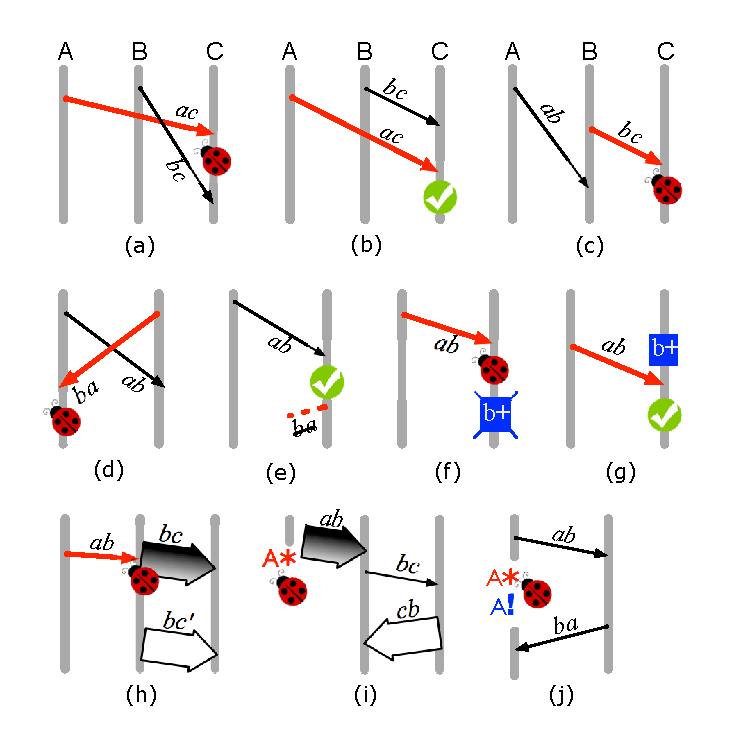
\includegraphics[width=3.5in]{F/patterns/basics.eps}
%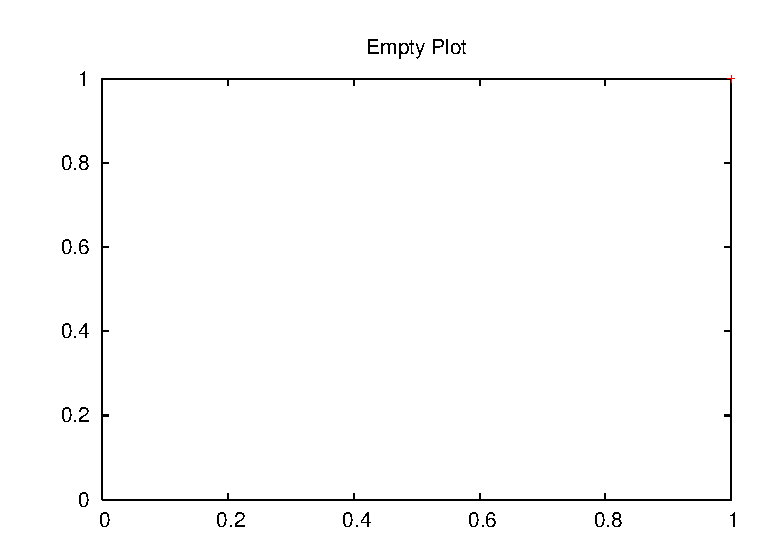
\includegraphics[width=0.5\textwidth]{F/empty.eps}
}
\vminten
\mycaption{pat}{Triggering patterns (\sec{\ref{trig-time}})}
{The three vertical lines represent the timeline of nodes A, B and C.
An arrow with \ts{xy} label implies a message from X to Y.  A square
box with label \ts{x+} implies a local state-modifying computation at
node X.  A thick arrow implies a set of messages performing an atomic
operation.  \ts{X*} and \ts{X!} implies a crash and reboot at node X
respectively (\sec\ref{met-pres}). All figures  are discussed in
\sec{\ref{trig-time}}}

\end{figure}



\if 0
\newtxt{The three lines represent
timeline of nodes A's, B's, and C's events (\ie\ sending/receiving
messages, local computations, crashes/reboots). Arrow lines ac mean
messages from A to C. Square boxes b+ mean local computations in B.
Thick arrows mean a set of messages doing an atomic operation. A*
means a crash of A, and A! means a reboot of A.  Figure (a)
illustrates an order violation pattern due to a race of two message
arrivals on node C (\ie\ messages ac/bc), which the bug would not
manifest if C receives the messages as in figure (b). Figures (c) and
(d) illustrate order violations between a message arrival and a
message sending (\ie\ ab/bc in (c), and ab/ba in (d)) which the bugs
would not happen if B receives the message ab before it sends a
message as in figure (e). Figure (f) illustrates an order violation
pattern between a message arrival and a local computation (\ie\ ab/b+)
which the bug would not manifest, if ab arrives after B has finished
b+ computation as in figure (g). Figure (h) illustrates an atomicity
violation that a message ab comes during B is doing an atomic
operation. Figure (i) illustrates a fault-timing pattern that A
crashes during an atomic operation (\ie\ A*/ab). Figure (j)
illustrates a reboot timing pattern that A crashes and reboots during
B processing a message ab, and A does not expect a message ba; the bug
would not happen if B tries to send ba and finds out A is dead. } }
\fi
 %----fig



% -------------------------
\paragraph{Fault and Reboot Timing Bugs.}

Fault and reboot timing bugs (\pctTrigFR\ in Table \ref{tab:trig})
manifest when faults and/or
reboots occur at specific global states $S$\sub{i}; the bugs do not
manifest if the faults and reboots happen at different global states
$S$\sub{j}. 

Figure \ref{pat}i illustrates a fault-timing bug in \mr{3858}.  Here,
A\sub{NM1} is sending a task's output to B\sub{AM} (\mab) but A
crashes in the middle (A*) leaving the output half-sent. 
The system is then unable to recover from this untimely crash --- B
detects the fault and reruns the task at C\sub{NM2} (via \mbc) and
later when C re-sends the output (\mcb), B throws an exception.  This
bug would not manifest, if the crash (A*) happens before/after
the output transfer (\mab).

Figure \ref{pat}j depicts a reboot-timing bug in \mr{3186}.  Here,
A\sub{RM} sends a job (\mab) to B\sub{AM} and while B is executing the
job, A crashes and reboots (A*, A!)  losing all its in-memory job
description.  Later, B sends a job-commit message (\mba) but A throws
an exception because A does not have the job information.  The bug
would not manifest if A reboots later: if A is still down when B sends
\mba\sub{commit} message, B will realize the crash and cancel the job before
A reboots and A will repeat the entire job assignment correctly.





\begin{figure}
\bugbox{
{\bf \zk{1264}:}
\enumerate{
\item \fev{Follower F crashed} in the past,
\item \fev{F reboots} and joins the cluster; then \fev{F synchronizes data} with Leader L
\item F sends FOLLOWERINFO message to L [synchronization message]
\item L sends LEADERINFO message to F [synchronization message]
\item F sends ACKEPOCH message to L [synchronization message]
\item L sends SNAP message to F [synchronization message]
\item L sends data tree snapshot to F [synchronization message]
\item L sends NEWLEADER message to F [synchronization message]
\item \fev{Client C sends a request} to update data with Tx-\#15 to L; L does atomic broadcast to update all followers
\item L sends update proposal message for Tx-\#15 to F [broadcast message]
\item F sends update ack message for Tx-\#15 to L [broadcast message]
\item \fev{L sends update commit message} for Tx-\#15 to F [broadcast message]
\item \fev{F applies the update} for Tx-\#15 to in-memory data tree, but not to on-disk log (because F has not received UPTODATE message)
\item \fev{L sends UPTODATE message} to F [synchronization message]
\item C sends a request to update data with Tx-\#16 to L
\item L sends update proposal for Tx-\#16 to F
\item F sends update ack for Tx-\#16 to L
\item L sends update commit for Tx-\#16 to F
\item F applies the update for Tx-\#16 to in-memory data tree and on-disk log
\item \fev{F crashes} (before \fev{F does snapshot})
\item F reboots and joins the cluster again
\item L synchronized data with F by sending update starting from Tx-\#17
\item F loses the update for Tx-15 C did in step 9
}
}
\mycaption[A DC bug in ZooKeeper]{fig-taxdc-zk1264}{A DC bug in ZooKeeper}{This figure shows Figure
\ref{fig-zk1264} again. It shows a DC bug in ZooKeeper that is caused from a mix
of untimely message arrivals and crash timing. This bug surfaces when a follower
receives update commit messasge (step 12) in the middle of an atomic operation
(step 3-14) and the follower crashes before it does snapshot (step 20)}
\end{figure}



%\ev{(5)} L forwards the update request txid \#15 to F,

% ---------------------------------------------------- CA simple
% ---------------------------------------------------- CA complex
% ---------------------------------------------------- HBase simple
% ---------------------------------------------------- HBase complex
% ---------------------------------------------------- MR simple
% ---------------------------------------------------- MR complex
% ---------------------------------------------------- ZK simple
% ---------------------------------------------------- ZK complex




\paragraph{Message-Fault Bugs.}
Four DC bugs are caused by a combination of messages and faults. 
For example, in Figure
\ref{fig-taxdc-zk1264}, a message (step 12) arrives in the middle of some
atomic operation (step 3-14). This message atomicity violation leads
to an error that further requires a fault timing (step 20) to become an
externally visible failure.



\finding{DC bugs are triggered mostly by 
\textit{untimely messages} (\pctTrigMsg\ in Table \ref{tab:trig}) 
and % $\sim$70\%
sometimes by \textit{untimely faults/reboots} (\pctTrigFR), % $\sim$30\% 
and occasionally by a \textit{combination} of both (\pctTrigMix). % $<$5\%
Among untimely messages, two thirds commit order violations 
% Some untimely messages commit order violations (\pctTrigMsgOrder), %\sim$60
due to message-message or message-computation race on the node they arrive;
%(Figure\ref{pat}a--g);
the others commit atomicity violations.}
%(Figure\ref{pat}h).}

%These patterns provide
%important guidance to future research in combating DC bugs
%(\ref{sec-sol}).
%}




% ===============================================
\subsection{Input Preconditions (IP)} 
\label{trig-input}


The previous section presents simple timing conditions that can be
understood in few simple steps.  In practice, many of the conditions
happen ``deep'' in system execution.  In other words, the triggering
path is caused by complex input preconditions (IP) such as faults, reboots,
and multiple protocols.  Let's use the same example in Figure
\ref{fig-taxdc-zk1264}.
%
First, a fault and a reboot (step 1-2) and a client request (step 9)
must happen to create a path to the message atomicity violation (step
9 interfering with step 3-14).
%
Second, conflicting messages from two different protocols (ZAB and
NodeJoin initiated in step 2 and 9) have to follow specific
bug-triggering timing conditions.
%
Even after the atomicity violation (after step 14), the bug is not
guaranteed to lead to any error yet (\ie, a benign race).
%
Finally, the follower experiences an untimely fault (step 20), such
that after it reboots (step 21), a global replica-inconsistency error
will happen (step 23).
%
Put it in a reverse way, before step 20, the global state is $S$\sub{i}
and $S$\sub{i}$+$crash$\rightarrow$error, and the only way for the
system to reach $S$\sub{i} is from complex preconditions such as a
fault, a reboot, and some foreground and background protocols.



Statistically, Figure \ref{bars}b (\BFLT) shows that \pctFaultYes\ of
DC bugs must have at least one fault.  In more detail, Figure
\ref{bars}c-e (\BTO, \BCR, \BRB) shows the percentage of issues that
require timeouts, crashes and reboots respectively, including how many
instances of such faults must be there; the rest is other faults such
as disk errors (not shown).


Figure \ref{bars}f (\BPROT) shows how many ``protocol initiations''
mentioned in the bug description.  For example, if the system needs to
perform one execution of background protocol and also three concurrent
calls to the \ts{write} protocol, then we label it with four protocol
initiations.  Up to 3 protocol initiations covers three quarters of
DC bugs.
%
When we count the number of {\em unique} protocols involved in all the
bugs we study, we record \totProtCA\ Cassandra, \totProtHB\ HBase,
\totProtMR\ MapReduce, \totProtZK\ ZooKeeper unique protocols, or
\totProtAll\ protocols in total.  This again highlights the complexity
of fully complete systems.
%
Figure \ref{bars}g (\BBFG) shows our categorization of protocols that
are concurrently running into foreground only,
background only, and foreground-background (mix)
categories.  More than three quarters of the bugs involve some
background protocols and about a quarter involves a mix of foreground
and background protocols.

\finding{Many DC bugs need \textit{complex input preconditions}, 
such as faults
(\pctFaultYes\ in Figure \ref{bars}b), multiple protocols
(\pctProtMany\ in Figure \ref{bars}f), and background protocols 
(\pctProtBg\ in Figure \ref{bars}g) .}







\begin{figure}

\centerline{
\begin{tikzpicture}[font=\sffamily\footnotesize]
\begin{axis}[
xbar stacked,
y=0.8cm,
width=3.375in,
width=\columnwidth,
%height=120pt,
xmin=0,
xmax=100,
bar width=12pt,  
%xmajorgrids=true,
%ylabel={Categorizations},
%symbolic y coords={TRIG, CD, PIN, IMP, REP, EM, RB, CR, TO, FLT, LM, TSM, TSP, TSN},
symbolic y coords={REP, FIX, IMP, EM, ES, ERR, TSU, TSP, TSN, TSM, PIN, SP, RB, CR, TO, FLT, TRIG},
ytick=data,
%yticklabels={{(n) TRIG, (m) CD, (l) PIN, (k) IMP, (j) REP, (i) EM, (h) RB, (g) CR, (f) TO, (e) FLT, (d) LM, (c) TSM, (b) TSP, (a) TSN}},
yticklabels={{(q) WHR, (p) FIX, (o) FAIL, (n) ER-E/S, (m) ER-L/G, (l) ERROR, (k) TS-UEv, (j) TS-PR, (i) TS-ND, (h) TS-MSG, (g) IP-B/F, (f) IP-PR, (e) IP-RB, (d) IP-CR, (c) IP-TO, (b) IP-FLT, (a) TC}},
every axis y label/.style={at={(ticklabel cs:0.5)},rotate=90,anchor=near ticklabel},
xticklabels={,,},
axis x line*=none,
x axis line style={opacity=0},
axis y line*=right
]
\addplot [fill=red!40] plot coordinates {(73.08,RB) (52.88,CR) (88.46,TO) (37.0,FLT)};
\addplot [fill=gray!40] plot coordinates {(20.19,RB) (34.62,CR) (11.54,TO) (63.0,FLT)};
\addplot [fill=pink!40] plot coordinates {(6.73,RB) (7.69,CR) (0,TO) (0,FLT)};
\addplot [fill=brown!40] plot coordinates {(0,RB) (4.81,CR) (0,TO) (0,FLT)};

\coordinate (rb0) at (36.54, -0.5);
\coordinate (rb1) at (83.175, -0.5);
\coordinate (rb2p) at (96.635, -0.5);
\coordinate (cr0) at (26.44, 99.5);
\coordinate (cr1) at (70.19, 99.5);
\coordinate (cr2) at (91.345, 99.5);
\coordinate (cr3p) at (97.595, 99.5);
\coordinate (toNo) at (44.23, 199.5);
\coordinate (toYes) at (94.23, 199.5);
\coordinate (fltNo) at (18.5, 299.5);
\coordinate (fltYes) at (68.5, 299.5);
\end{axis}

\node at (rb0) {0 (73\%)};
\node at (rb1) {1 (20\%)};
\node at (rb2p) {2+};
\node at (cr0) {0 (53\%)};
\node at (cr1) {1 (35\%)};
\node at (cr2) {2 (8\%)};
\node at (cr3p) {3+};
\node at (toNo) {No (88\%)};
\node at (toYes) {Yes (12\%)};
\node at (fltNo) {No (37\%)};
\node at (fltYes) {Yes (63\%)};

\end{tikzpicture}
%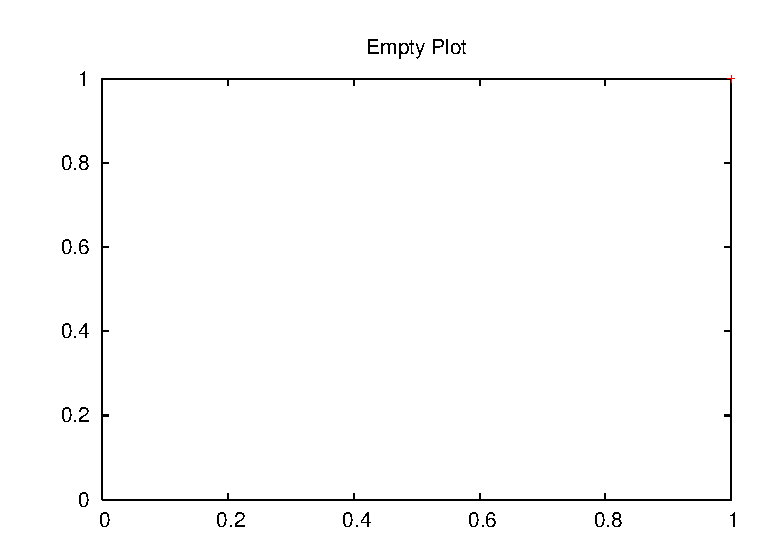
\includegraphics[width=1.8in]{F/empty.eps}
}
\vminten
\mycaption{bars}{Statistical overview of \tdc}
{Timing Conditions (TC) is discussed in \sec\ref{trig-time},
Input Preconditions (IP) in \sec\ref{trig-input},
Triggering Scope (TS) in \sec\ref{trig-scope},
Errors (ER) in \sec\ref{err-err},
Failures (FAIL) in \sec\ref{err-fail},
Fixes (FIX) in \sec\ref{sec-fix},
and Where Found (WHR) in \sec\ref{sec-stat}.}
% \vten

\end{figure}


%
\if 0
nodes (TSN), 
protocols (TSP), 
background (BR), 
triggering messages (TSM), 
local-message race (LM), 
timeout (TO),
crashes (CR),
reboots (RB),
errorMessage (EM),
reported (REP),  
implication (IMP),
control/data plane (CDP), 
\fi



\begin{figure*}

\centerline{
%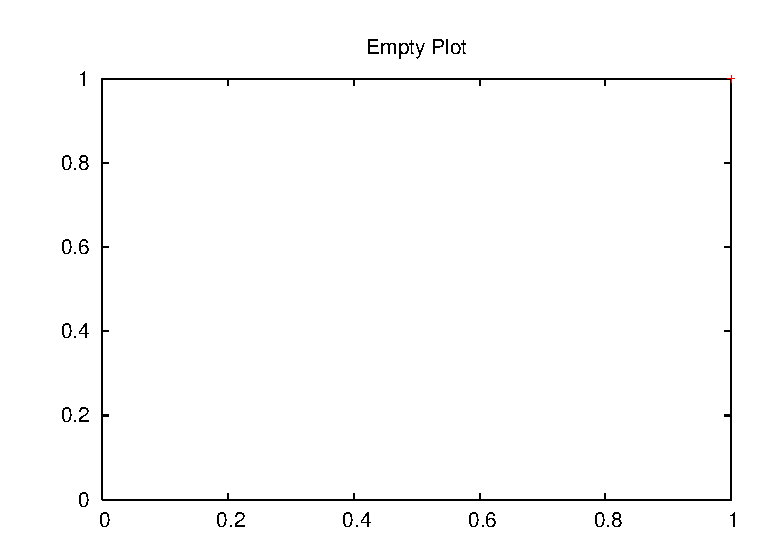
\includegraphics[width=6.5in]{F/empty.eps}
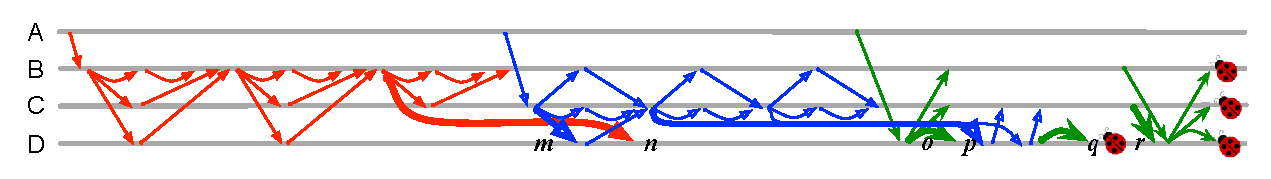
\includegraphics[width=7.0in]{F/paxos/paxos.eps}%
}
\vminfive
\mycaption[A Cassandra's Paxos bug]{fig-paxos}{A Cassandra's Paxos bug}{In \ca{6023}, 
three key-value updates 
(different arrow types)
concurrently execute the Paxos protocol on four nodes
(we simplify from the actual six nodes).
The bug requires three message-message race conditions:
(1) \emph{m} arrives before \emph{n}, 
(2) \emph{o} before \emph{p}, and
(3) \emph{q} before \emph{r}, which collectively
makes D corrupt the data and propagate the corruption
to all replicas after the last broadcast.
Note that the bug would not surface if any of the conditions
did not happen. 
It took us one full day to study this bug.
}
\vten
\end{figure*}

 % --

\if 0
\pctProtMany\ \xxx\ of the bugs must
have at least two different protocols running.  A protocol sometimes
must also be triggered multiple times (\eg, three clients concurrently
run the \ts{write} protocol), but currently we do not track this
number.  
\fi


\vten


% ===============================================
\subsection{Triggering Scope (TS)}
\label{trig-scope}


We now analyze the triggering scope (TS), which is a complexity measure of
DC-bug timing conditions.  We use four metrics to measure the scope:
message count (\BTSM), node (\BTSN), protocol (\BTSP), and untimely
event (\BTSU) counts as shown in Figure \ref{bars}h-k.  This statistic
is important with respect to the scalability of model checking, bug
detection and failure diagnostic tools
(\sec\ref{less-dmck}-\ref{less-diagnose}).

Message count implies the minimum
number of messages involved in $E$ as defined in the beginning of
section \ref{sec-trig}.  Figure \ref{bars}h (\BTSM) shows that one or two
triggering messages are the most common, with 7 messages as the
maximum.  Informally, zero implies fault timing bugs without any
message-related races, one implies message-compute race, two implies
message-message as in Figure \ref{pat}a, and three implies a scenario
such as \mac/(\mab-\mbc) race where \mab\ and \mac\ are concurrent or
non-blocking message sending operations.

The node and protocol scopes present how many nodes and protocols are
involved within the message scope.  Figure \ref{bars}i-j (\BTSN\ and
\BTSP) shows that the scale of node and protocol triggering scope is
also small, mostly two or three nodes and one or two protocols.

The untimely events count implies the total number of order
violations, atomicity violations, untimely faults and reboots in the
triggering timing condition of a bug.  Figure \ref{bars}k
(\BTSU) shows that only eight bugs require more than one untimely
events.  Four of them are message-fault bugs, each 
requiring one untimely message and one
untimely fault to trigger (\eg, step 9 and 20 in 
Figure \ref{fig-taxdc-zk1264}).  Three are fault-reboot timing bugs,
each requiring one untimely fault and one untimely reboot.
The last one is \ca{6023}, shown in Figure \ref{fig-paxos}, requiring
three message-message order violations to happen.

%TODO
% --- after the occurrence of 
%the one untimely event, the first error will deterministically propagate to
%failures

\finding{The \textit{timing conditions} of most DC bugs only involve 
\textit{one to three} messages, nodes, and protocols ($>$90\% in
Figure \ref{bars}h-j).  Most DC bugs are mostly triggered by 
only \textit{one} untimely event (\pctTrigScopeUnEvOne\ in Figure 
\ref{bars}k).}
%, which
%is a positive finding for the scalability of
%future bug finding tools (\sec\ref{less-bft}).
%Furthermore, more focus on interactions between foreground
%and background protocols that involve control logic should
%be exercised. 

